\chapter{Výsledky}\label{chap:results}
V tejto kapitole si priblížime metodiku testovania nášho riešenia, opíšeme si testovacie scenáre a zosumarizujeme výsledky ktoré boli dosiahnuté. Taktiež sa zameriame na opis možných vylepšení a návrh prípadnej budúcej práce na rozšírení grafického editora. V závere tejto kapitoly sa nachádzajú ukážky používateľského prostredia grafického editora a spôsobu integrácie do systému MediaWiki.

\section{Testovanie}
Počas aktívneho vývoja aplikácie bolo zorganizované skupinové záťažové testovanie. Zúčastnili sa na ňom študenti prvého ročníka vysokej školy v počte 6. ľudí. V čase testovania bola aplikácia v stave tesne pred dokončením a obsahovala niekoľko chýb, o ktorých boli testujúci účastníci oboznámený. Testovanie prebiehalo v dvoch krokoch. V prvom kroku testovala aplikáciu skupina 3. používateľov ktorý pracovali na zadaní popísanom v testovacom scenári nižšie. V druhom kroku bol použitý záťažový test, kedy všetci používatelia testovali aplikáciu súčastne, s veľkým počtom operácií za účelom zistenia stability synchronizácie editora.

\subsection{Testovací scenár}
Zadaním testovacieho scenára bolo \textit{vytvoriť jednoduchý grafický návrh webovej aplikácie} vo forme blogu. Grafický návrh musel pozostávať z 3. podstránok.
\begin{enumerate}
	\item \textit{Hlavná stránka} so zoznamom blogov(článkov), obsahujúca zoznam jednotlivých článkov blogu s nadpisom, dátumom, obrázkom, autorom a tlačidlami stránkovania zoznamu.
	\item \textit{Stránka konkrétneho článku} s nadpisom, úvodným obrázkom a ľubovoľným obsahom.
	\item \textit{Profil autora blogu} s jeho aktivitou.
\end{enumerate}

\subsection{Výsledky testovania}
Pri testovaní sa neprejavili žiadne zásadné nedostatky alebo chyby aplikácie, okrem tých, na ktoré boli účastníci upozornený. V jednom prípade sa nepodarilo načítať prostredie grafického editora, čo bolo spôsobené zastaralou verziou internetového prehliadača. 

Zúčastnená vzorka používateľov bola po testovaní vyzvaná na vyplnenie krátkeho dotazníka, kde bolo potrebné zhodnotiť prácu s editorom a popísať jeho prípadné nedostatky. 

Intuitívnosť ovládania zhodnotili používatelia pozitívne. Synchronizácia aplikácií editorov jednotlivých používateľov prebiehala taktiež bez problémov. Za najväčší nedostatok bolo popísané chýbajúce tlačidlo na krok späť. Ostatné nedostatky boli po testovaní zapracované alebo opravené.

\section{Návrhy na vylepšenie a budúcu prácu}
Tak ako sa prejavilo pri testovaní, najväčším nedostatkom editora je návrat vykonaných zmien používateľom. Ide však o veľmi kľúčovú funkcionalitu, ktorú pri aktuálnom spôsobe implementácie nieje možné jednoducho zapracovať a vyžadovala by si dlhší čas potrebný na zapracovanie. Preto je to jedno z možných budúcich vylepšení. 

Ďalším možným vylepšením je lepšie rozčlenenie zdrojových súborov do samostatných tried. To by zlepšilo prehľadnosť zdrojového kódu a jeho jednoduchšiu rozšíriteľnosť. 

Knižnica Fabric poskytuje funkcionalitu na aplikovanie grafických filtrov na objekty typu obrázok. Zapracovanie tejto funkcionality do grafického editora by taktiež značne zvýšilo jeho použiteľnosť.

\section{Ukážky prostredia editora obrázkov}

\begin{figure}
	\centering
	\begin{subfigure}[t]{0.48\linewidth}	
		\centerline{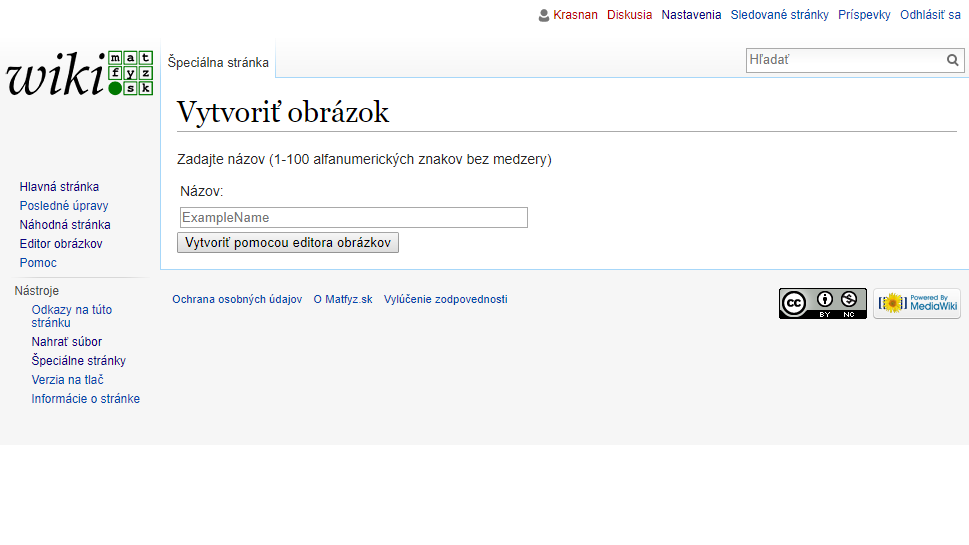
\includegraphics[width=1\textwidth]{images/results/base-new}}
		\caption{Vytvorenie nového obrázka}
	\end{subfigure}
	\quad
	\begin{subfigure}[t]{0.48\linewidth}	
		\centerline{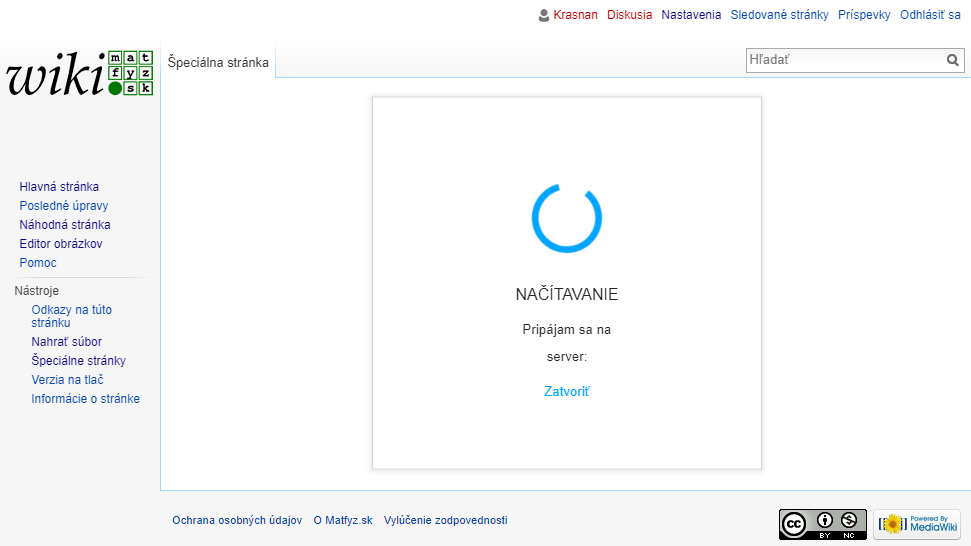
\includegraphics[width=1\textwidth]{images/results/base-loading}}
		\caption{Zobrazenie načítavania}
	\end{subfigure}
	\quad
	\begin{subfigure}[t]{1\linewidth}	
		\centerline{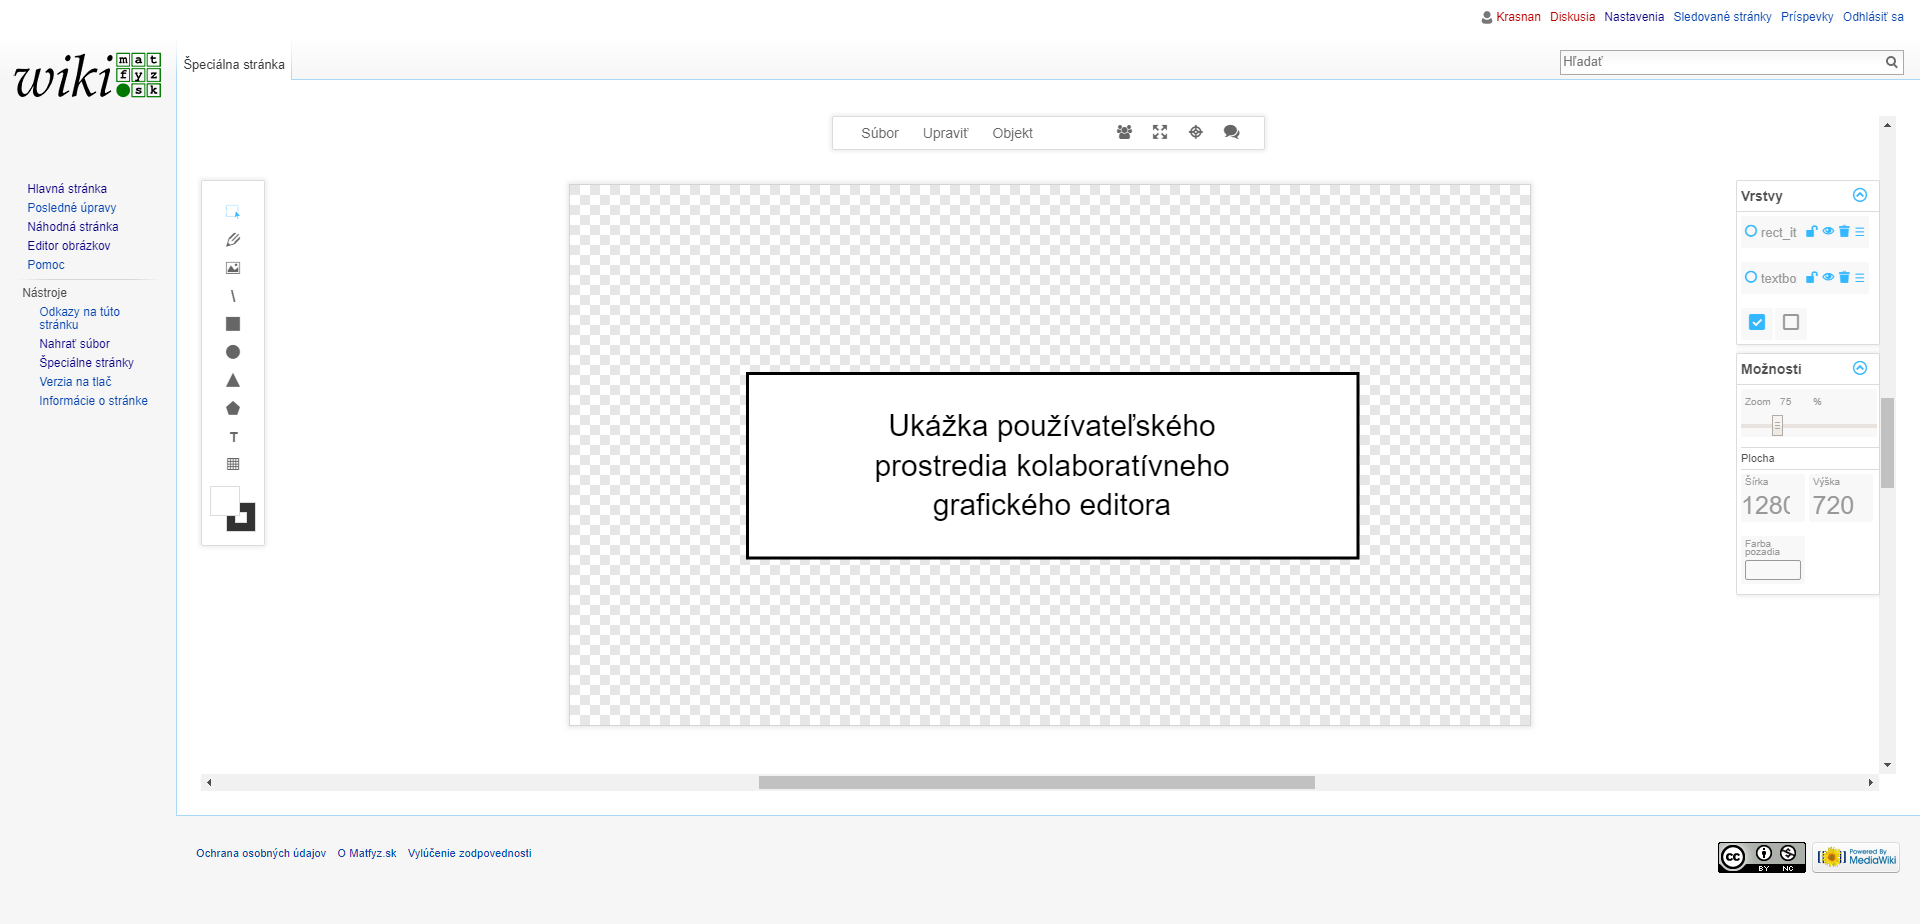
\includegraphics[width=1\textwidth]{images/results/base-editor}}
		\caption{Používateľské prostredie editora obrázkov}
	\end{subfigure}
	\quad
	\begin{subfigure}[t]{1\linewidth}	
		\centerline{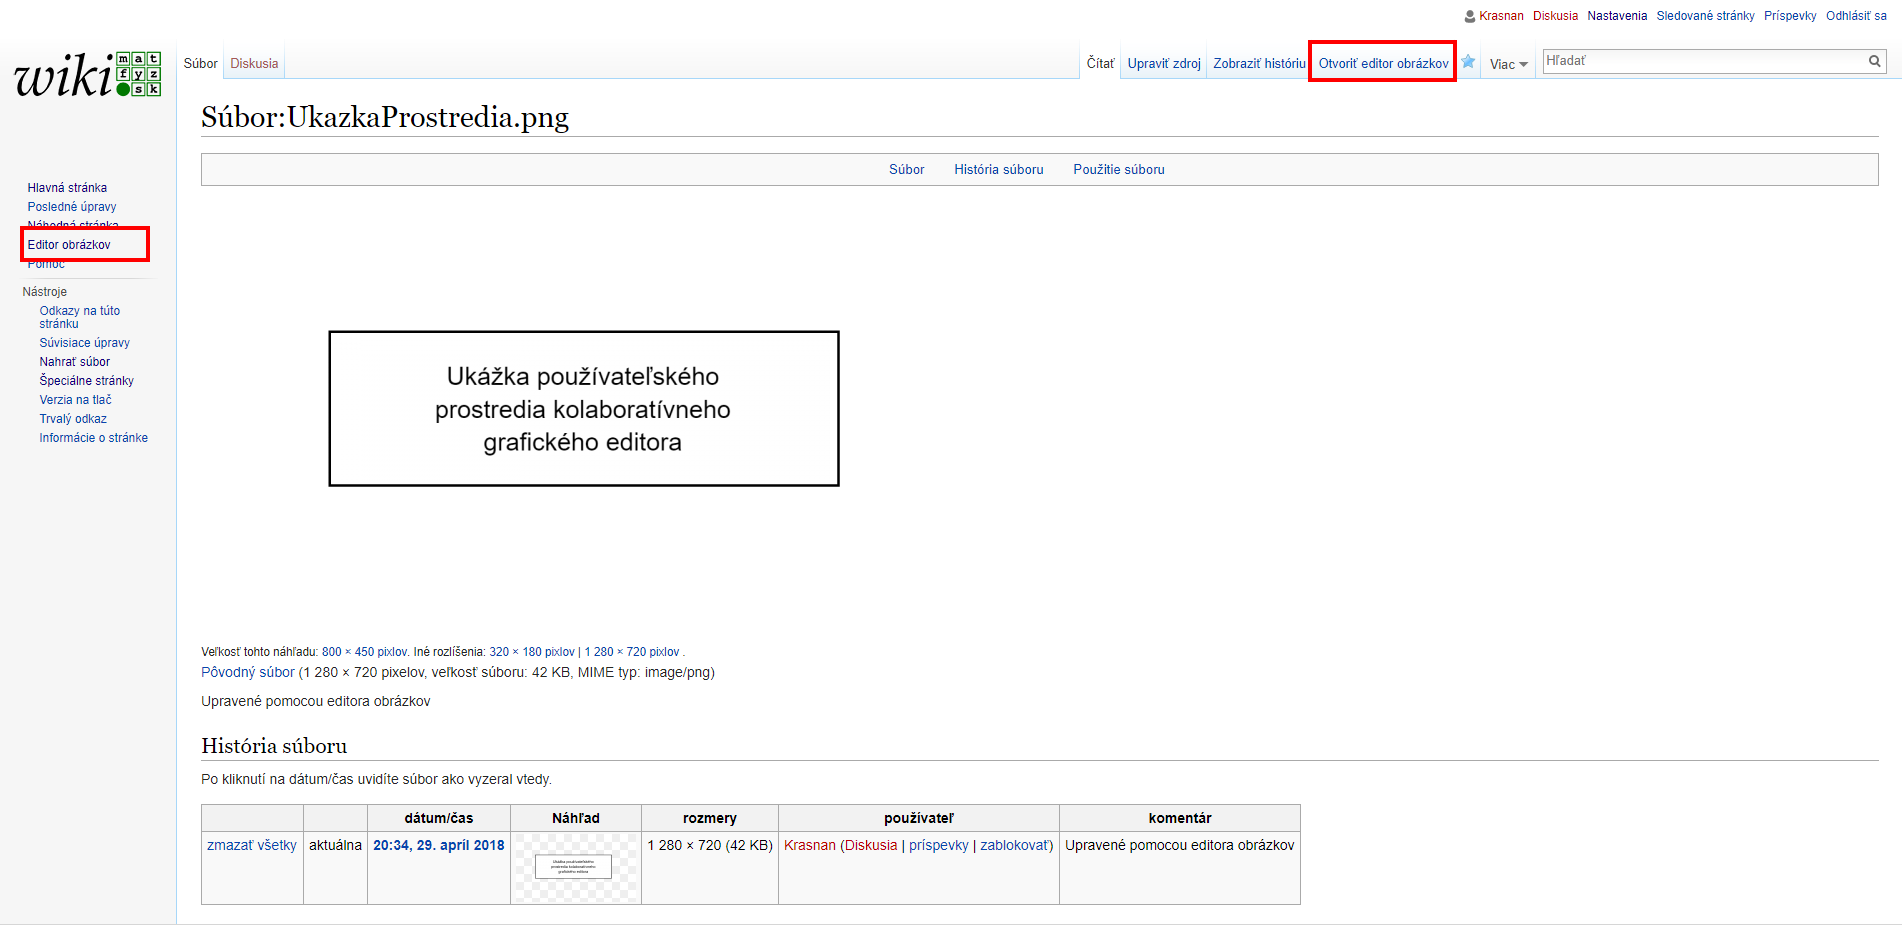
\includegraphics[width=1\textwidth]{images/results/base-integration}}
		\caption{Integrácia do systému MediaWiki}
	\end{subfigure}
	\caption{Používateľské prostredie rozšírenia}
\end{figure}


\begin{figure}
	\centering
	\begin{subfigure}[t]{0.48\linewidth}	
		\centering{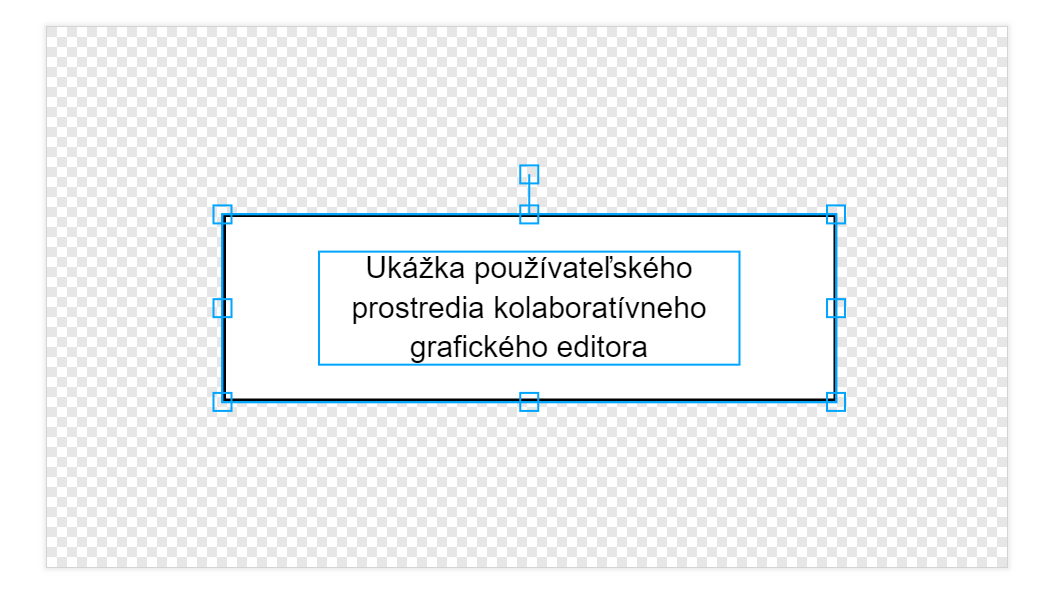
\includegraphics[width=1\textwidth]{images/results/canvas-selected}}
		\caption{Označenie aktívnych objektov}
	\end{subfigure}
	\quad
	\begin{subfigure}[t]{0.48\linewidth}	
		\centering{
\includegraphics[width=1\textwidth]{images/results/canvas-locked}}
		\caption{Zobrazenia používateľa, ktorý uzamkol objekt}
	\end{subfigure}
	
	\caption{Uzamykanie objektov}
\end{figure}


\begin{figure}
	\centering
	\begin{subfigure}[t]{0.48\linewidth}	
		\centering{
\includegraphics[width=1\textwidth]{images/results/dialog-upload}}
		\caption{Dialógové okno na nahratie súboru}
	\end{subfigure}
	\quad
	\begin{subfigure}[t]{0.48\linewidth}	
		\centering{
\includegraphics[width=1\textwidth]{images/results/dialog-delete}}
		\caption{Dialógové okno na potvrdenie vymazania grafického objektu}
	\end{subfigure}
	\quad
	\begin{subfigure}[t]{0.7\linewidth}	
		\centering{
\includegraphics[width=1\textwidth]{images/results/dialog-close}}
		\caption{Dialógové okno zobrazené pri zatváraní editora}
	\end{subfigure}
	
	\caption{Dialógové okná}
\end{figure}


\begin{figure}
	\centering
	\begin{subfigure}[t]{0.48\linewidth}	
		\centering{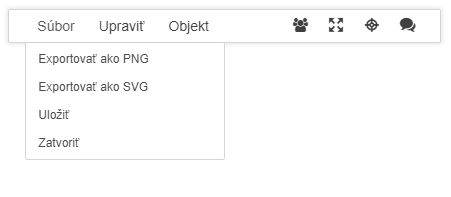
\includegraphics[width=1\textwidth]{images/results/menu-file}}
		\caption{Rozbaľovacie menu pre tlačidlo \textit{Súbor}}
	\end{subfigure}
	\quad
	\begin{subfigure}[t]{0.48\linewidth}	
		\centering{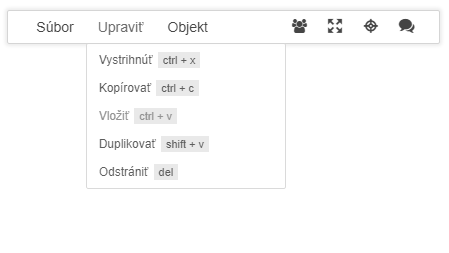
\includegraphics[width=1\textwidth]{images/results/menu-edit}}
		\caption{Rozbaľovacie menu pre tlačidlo \textit{Upraviť}}
	\end{subfigure}
	\quad
	\begin{subfigure}[t]{0.48\linewidth}	
		\centering{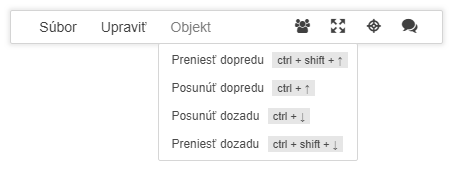
\includegraphics[width=1\textwidth]{images/results/menu-object}}
		\caption{Rozbaľovacie menu pre tlačidlo \textit{Objekt} }
	\end{subfigure}
	\quad
	\begin{subfigure}[t]{0.48\linewidth}	
		\centering{
\includegraphics[width=1\textwidth]{images/results/menu-users}}
		\caption{Rozbaľovacie menu zoznamu pripojených používateľov  }
	\end{subfigure}
	\quad
	\begin{subfigure}[t]{0.6\linewidth}	
		\centering{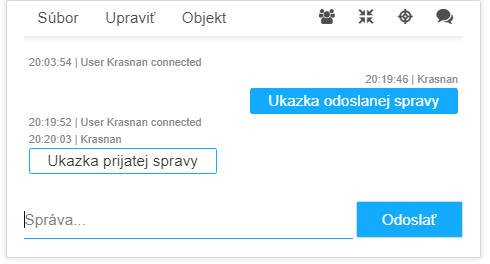
\includegraphics[width=1\textwidth]{images/results/menu-messenger}}
		\caption{Prostredie pre odosielanie textových správ}
	\end{subfigure}
	\caption{Zobrazenie hlavného menu}
\end{figure}


\begin{figure}
	\centering
	\begin{subfigure}[t]{0.48\linewidth}	
		\centering{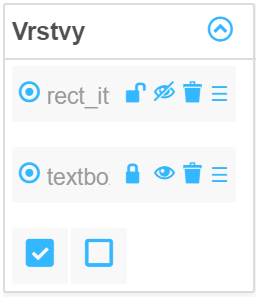
\includegraphics[height=6cm]{images/results/props-layers}}
		\caption{Panel vrstiev }
	\end{subfigure}
	\quad
	\begin{subfigure}[t]{0.48\linewidth}	
		\centering{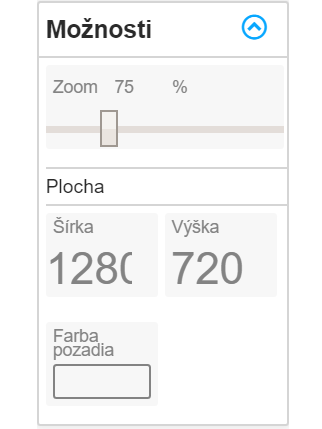
\includegraphics[height=6cm]{images/results/props-canvas}}
		\caption{Panel nastavení grafickej plochy}
	\end{subfigure}
	\quad
	\begin{subfigure}[t]{0.48\linewidth}	
		\centering{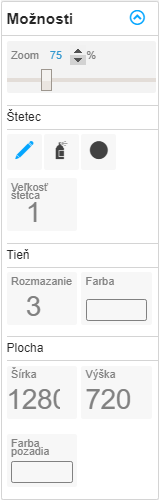
\includegraphics[height=6cm]{images/results/props-brush}}
		\caption{Panel nastavení voľného kreslenia}
	\end{subfigure}
	\quad
	\begin{subfigure}[t]{0.48\linewidth}	
		\centering{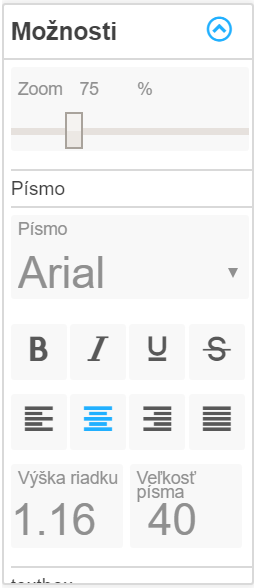
\includegraphics[height=6cm]{images/results/props-text}}
		\caption{Panel nastavení textového objektu}
	\end{subfigure}
	\quad
	\begin{subfigure}[t]{0.48\linewidth}	
		\centering{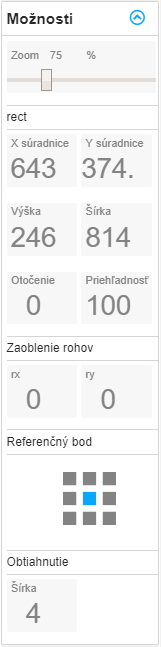
\includegraphics[height=7cm]{images/results/props-object}}
		\caption{Panel nastavení objektu}
	\end{subfigure}
	\caption{Ukážka panelov s nastaveniami}
\end{figure}

